\documentclass[11pt]{article}

\usepackage{amsmath}
\usepackage{graphicx}
\usepackage{indentfirst}
\usepackage{tabularx}
\usepackage{booktabs}
\usepackage[table]{xcolor}
\usepackage{subfiles}
\usepackage{setspace}
\usepackage{lipsum}
\usepackage{float}
\usepackage{comment}
\usepackage{hyperref}
\usepackage{caption}
\usepackage{tocloft}
\usepackage{subcaption}
\hypersetup{
    colorlinks=true,
    linkcolor=black,
    filecolor=magenta,      
    urlcolor=cyan,
    pdfpagemode=FullScreen,
}

\renewcommand{\cftsecleader}{\cftdotfill{\cftdotsep}}

\graphicspath{{images/}{../images/}}

\addtolength{\oddsidemargin}{-.5in}
\addtolength{\evensidemargin}{-.5in}
\addtolength{\textwidth}{1in}

\addtolength{\topmargin}{-.5in}
\addtolength{\textheight}{1in}

\definecolor{myred}{RGB}{243, 220, 219}
\definecolor{myblue}{RGB}{218, 238, 242}

%-----------------------------------------------------------

\begin{document}\errorcontextlines=9
\onehalfspacing

\begin{center}
\MakeUppercase{Catholic University of the Sacred Heart\\
Interfaculty of Mathematics, Physics and Natural Sciences\\
Applied Data Science for Banking and Finance}\\
\vspace{1cm}
Teaching Assistant: Peter Cincinelli \\
\vspace{24pt}
\huge Portfolio Analysis with \\ Fama \& French \& Carhart Model\\
\vspace{144pt}
\LARGE Authors: \\ 
\large Borgo Riccardo\\
Santucci Edoardo\\
Moe David Alexander \\
Kolbasov Maksim\\
Medvedieva Kateryna\\
\end{center}

\pagenumbering{gobble}
\clearpage
\tableofcontents
\clearpage
\listoffigures
\clearpage
\listoftables
\clearpage

\pagenumbering{arabic}

\section{Introduction}

The aim of this report is to analyze a set of ten portfolios composed by unknown UK stocks applying the Fama\&French\&Carhart model with the purpose of studying the 
different portfolios and comparing them.\\
We have been provided with a monthly data from October 1980 to December 2010 containing:
\begin{enumerate}
    \item The returns of the ten UK portfolios. Stocks have been assigned to portfolios based on their market capitalization, so that the stocks of the companies with the 
    smallest capitalization are in S1 and the stocks of the companies with the largest capitalization are in S10;
    \item The four risk factors of the Fama\&French\&Carhart model (SMB, HML, UMD and RMRF);
    \item The risk-free return.
\end{enumerate}

%------Descriptive Statistics------%

\section{Descriptive Statistic}
Firstly, we calculated the excess return for each portfolio as portfolio return minus the UK risk-free return.
\begin{figure}[H]
    \begin{center}
        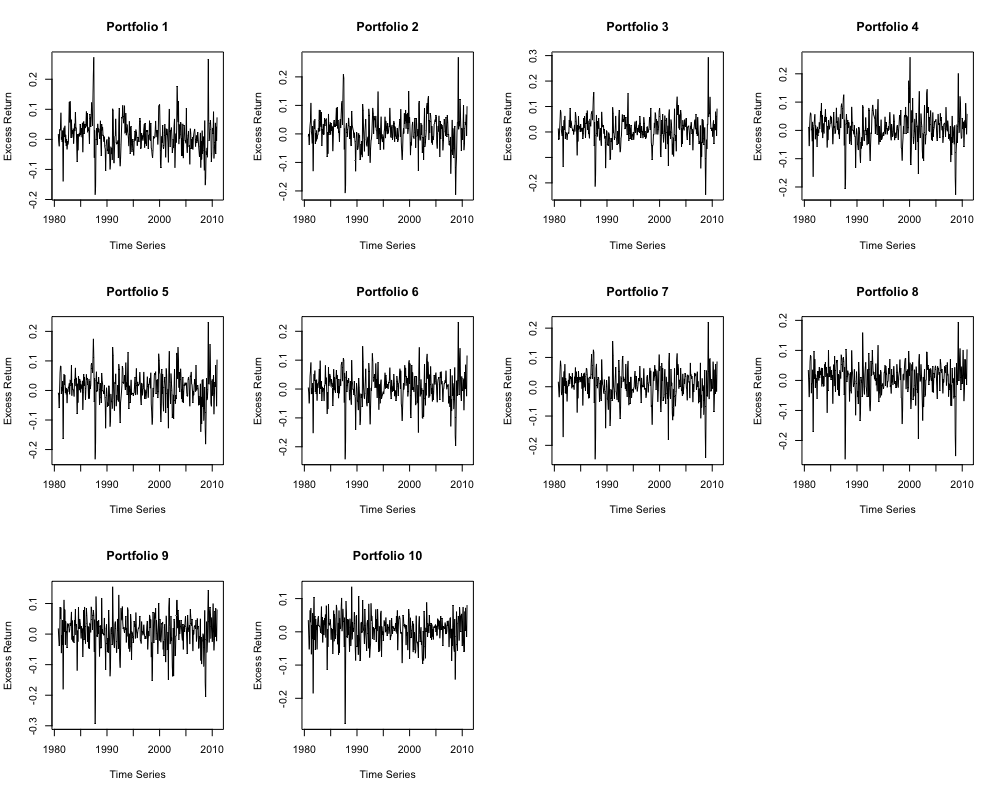
\includegraphics[scale = .3]{excess_returns_time.png}
    \end{center}
    \caption{Excess Returns of every portfolio from 1980 to 2010}
    \label{fig:excess_port}
\end{figure}
The figure \textbf{\ref{fig:excess_port}} shows the excess returns for every portfolio.\\
The problem is that it is very difficult to compare the excess returns on these graphs. We can see that they all follow almost the same trend.
As a consequence we decided to calculate the portfolio's cumulative excess returns to understand how much pounds we will receive at the end of 2010 if we invest 1 pound in October 1980. The figure 2 illustrates the given result.
The cumulative excess return was calculated as follows:
\begin{equation}
    (1 + R_1)(1 + R_2)\hdots(1 + R_n) - 1 
    \label{eq:equation_excess}
\end{equation}
where R\textsubscript{1} - return of the first period - October1980,\\
R\textsubscript{2} - return of the second period - November 1980,\\
R\textsubscript{n} - return of the last period - December 2010.

\begin{figure}[H]
    \begin{center}
        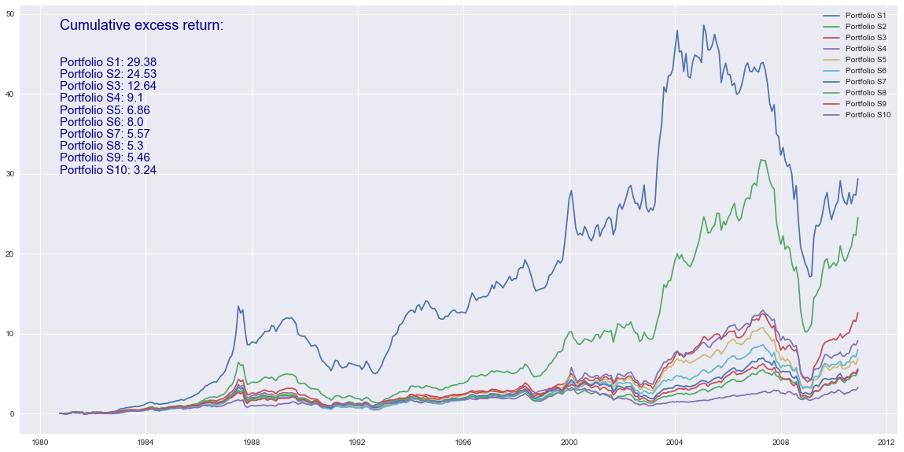
\includegraphics[scale = .9]{cumulative_excess_returns.png}
    \end{center}
    \caption{Cumulative excess returns of every portfolio from 1980 to 2010}
    \label{fig:cum_excess_port}
\end{figure}

Now we can easily see the difference between the portfolios. We can say, for example, that our 1 pound invested in October 1980 in the portfolio S1 will give us at 
the end of December 2010 29,38 pounds more than if we would invest in the UK risk free portfolio. Likewise, 1 pound invested in the portfolio S10 - only 3.24 pounds excess. 
The final excess return (as December 2010) is depicted on the figure \textbf{\ref{fig:fin_excess_port}}.
\begin{figure}[H]
    \begin{center}
        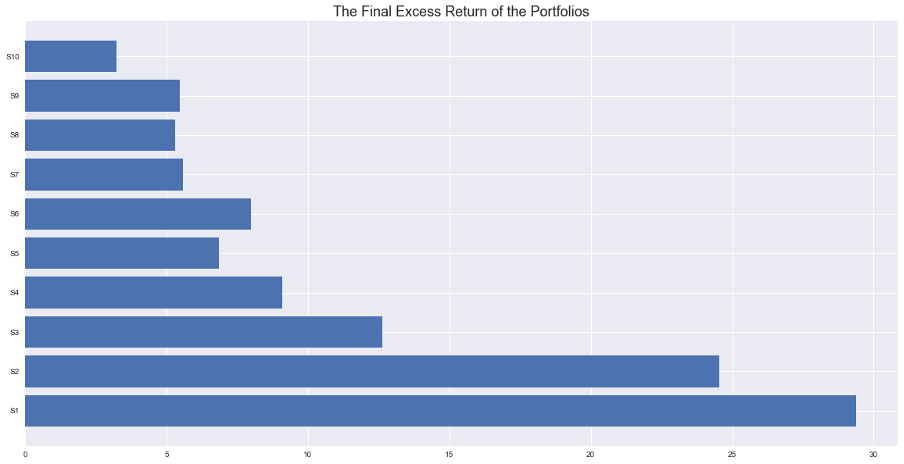
\includegraphics[scale = .9]{bar_excess_returns.png}
    \end{center}
    \caption{Final Excess Return for every portfolio}
    \label{fig:fin_excess_port}
\end{figure}

Another aspect we can notice from figure \textbf{\ref{fig:cum_excess_port}} is the high volatility of portfolio S1 and a lower one for portfolio S10.\\
Another thing we did is the transformation of our monthly data into years because we are more accustomed to annual interest than to monthly interest. 
Then we want to see how the different portfolios behaved in the different years. We eliminated the data for 1980 (as there are only 3 months from October to December). 
The excess return for every year was calculated as follows:
\begin{equation}
    (1 + R_1)(1 + R_2)\hdots(1 + R_{12}) - 1
\end{equation}
where R\textsubscript{1} is the excess return in January, and R\textsubscript{12} is the excess return in December.
The results are in the table \textbf{\ref{tab:month_year_er}}.
\begin{table}[H]
    \centering
    \begin{tabular}{ccccccccccc}
    \toprule\toprule
    & \textbf{XS1} & \textbf{XS2} & \textbf{XS3} & \textbf{XS4} & \textbf{XS5} & \textbf{XS6} & \textbf{XS7} & \textbf{XS8} & \textbf{XS9} & \textbf{XS10}\\ 
    \midrule
    1981 & 13\% & 11\% & 14\% & 6\% & 16\% & 9\% & 6\% & 12\% & 5\% & 1\% \\
    1982 & 20\% & 10\% & 3\% & -1\% & 3\% & 19\% & 11\% & 13\% & 20\% & 16\% \\
    1983 & 52\% & 35\% & 29\% & 40\% & 27\% & 9\% & 22\% & 22\% & 21\% & 21\% \\
    1984 & 17\% & 16\% & 19\% & 21\% & 18\% & 17\% & 23\% & 24\% & 22\% & 19\% \\ 
    1985 & 41\% & 21\% & 18\% & 16\% & 10\% & 13\% & 15\% & 11\% & 11\% & 5\% \\ 
    1986 & 74\% & 52\% & 40\% & 28\% & 24\% & 27\% & 25\% & 21\% & 22\% & 13\% \\
    1987 & 62\% & 41\% & 17\% & 19\% & 27\% & 13\% & 11\% & 8\% & 5\% & -2\% \\
    1988 & 17\% & 8\% & 4\% & 3\% & 9\% & 6\% & 5\% & 6\% & 2\% & 2\% \\
    1989 & -5\% & -7\% & -5\% & -6\% & -10\% & -6\% & -6\% & 2\% & 7\% & 22\% \\
    \rowcolor{myred} 1990 & -36\% & -39\% & -40\% & -41\% & -39\% & -37\% & -36\% & -31\% & -27\% & -19\% \\
    1991 & 4\% & 0\% & 1\% & 0\% & 9\% & 8\% & 16\% & 10\% & 3\% & 11\% \\
    1992 & 0\% & -15\% & -7\% & -2\% & -2\% & -3\% & -1\% & 4\% & 18\% & 9\% \\
    1993 & 93\% & 55\% & 55\% & 61\% & 46\% & 46\% & 35\% & 22\% & 29\% & 15\% \\
    1994 & 4\% & 10\% & 6\% & -6\% & 2\% & -8\% & -6\% & -9\% & -9\% & -9\% \\
    1995 & -3\% & 13\% & 9\% & 4\% & 17\% & 17\% & 12\% & 9\% & 15\% & 13\% \\
    1996 & 15\% & 24\% & 9\% & 7\% & 12\% & 16\% & 13 & 13\% & 12\% & 7\% \\
    1997 & 14\% & 3\% & 5\% & -1\% & 6\% & 3\% & 6\% & 4\% & 0\% & 16\% \\
    1998 & -7\% & -5\% & -12\% & -11\% & -17\% & -10\% & -9\% & -17\% & -12\% & 12\% \\
    \rowcolor{myblue} 1999 & 51\% & 86\% & 51\% & 93\% & 64\% & 59\% & 47\% & 46\% & 37\% & 12\% \\
    2000 & -8\% & -3\% & -1\% & 13\% & -7\% & 5\% & 0\% & -10\% & 4\% & -11\% \\
    2001 & 18\% & 18\% & 5\% & 7\% & 11\% & 3\% & -4\% & -11\% & -4\% & -22\% \\
    \rowcolor{myred} 2002 & -1\% & -12\% & -13\% & -15\% & -21\% & -24\% & -28\% & -23\% & -33\% & -27\% \\
    \rowcolor{myblue} 2003 & 64\% & 77\% & 62\% & 60\% & 68\% & 41\% & 31\% & 34\% & 37\% & 16\% \\
    2004 & 3\% & 20\% & 27\% & 16\% & 13\% & 14\% & 18\% & 18\% & 22\% & 6\% \\
    2005 & -1 & 8\% & 12\% & 19\% & 16\% & 24\% & 22\% & 25\% & 22\% & 18\% \\
    2006 & -2\% & 20\% & 19\% & 16\% & 22\% & 23\% & 25\% & 25\% & 23\% & 12\% \\
    2007 & -18\% & -21\% & -23\% & -14\% & -23\% & -20\% & -13\% & -7\% & -10\% & 12\% \\
    \rowcolor{myred} 2008 & -45\% & -52\% & -46\% & -51\% & -49\% & -42\% & -45\% & -45\% & -46\% & -25\% \\
    \rowcolor{myblue} 2009 & 28\% & 74\% & 92\% & 46\% & 49\% & 69\% & 48\% & 56\% & 51\% & 28\% \\
    2010 & 20\% & 31\% & 34\% & 28\% & 19\% & 26\% & 22\% & 32\% & 30\% & 14\% \\
    \midrule
    \midrule
    Mean & 16,1\% & 15,9\% & 12,8\% & 11,9\% & 10,7\% & 10,6\% & 9,0\% & 8,8\% & 8,8\% & 6,1\% \\
    SD & 31,2\% & 31,6\% & 28,6\% & 29,0\% & 26,2\% & 24,6\% & 21,6\% & 21,8\% & 21,3\% & 14,5\% \\
    IQR & 28,0\% & 31,3\% & 25,0\% & 23,0\% & 22,1\% & 23,5\% & 26,1\% & 26,7\% & 24,5\% & 14,1\% \\
    \bottomrule
    \bottomrule
    \end{tabular}
    \caption{Excess Return of every portfolio by year} 
    \label{tab:month_year_er}
\end{table}

The top 3 years (with the biggest excess returns), 1999, 2003 and 2009, are colored in blue, and the worst 3 years, 1990, 2002 and 2008, are colored in red. 
In 1990 there was a recession which began in July 1990 and ended in March 1991. This recession was sparked by Iraq's invasion of Kuwait in the summer of 1990. 
In 2002 burst the dot-com bubble formed as a result of a surge of investments in the internet and technology stocks. Massive amounts of venture capital were dumped 
into tech and internet startups, while investors purchased shares in these companies on the hope of success. The crash wiped out \$5 trillion U.S. in technology-firm 
market value between March and October of 2002. Finally the financial crisis of 2007-2008 (figures 4 and 5). It was an epic financial and economic collapse that cost 
many ordinary people their jobs, their life savings, their homes, or all three.\\
At the bottom of the table we can see the descriptive statistics for the 10 portfolios. The largest average excess return over the years is the portfolio 
S1 - average excess return is 16.1\% while portfolio S10 is only 6.1\% on average. But we also need to consider the risk. The most profitable portfolio, 
S1, has the second largest volatility (-31.2\%) which means that with 68\% probability of expected excess return can roughly vary between (-15.1\%) and 47.3\%. 
The 95\% confidence interval of the expected excess return is [-46.3\%,78.5\%]. The portfolio S10 has the lowest risk (14.5\%), more than two times smaller compared to S1.\\
To compare the excess return over the years we present the portfolio with the smallest capitalization and the biggest cap - figures \textbf{\ref{fig:ex_ret_by_years1}} and 
\textbf{\ref{fig:ex_ret_by_years10}} - portfolio S1 and S10 respectively.

\begin{figure}[H]
    \centering
    \begin{subfigure}[b]{0.5\textwidth}
        \centering
        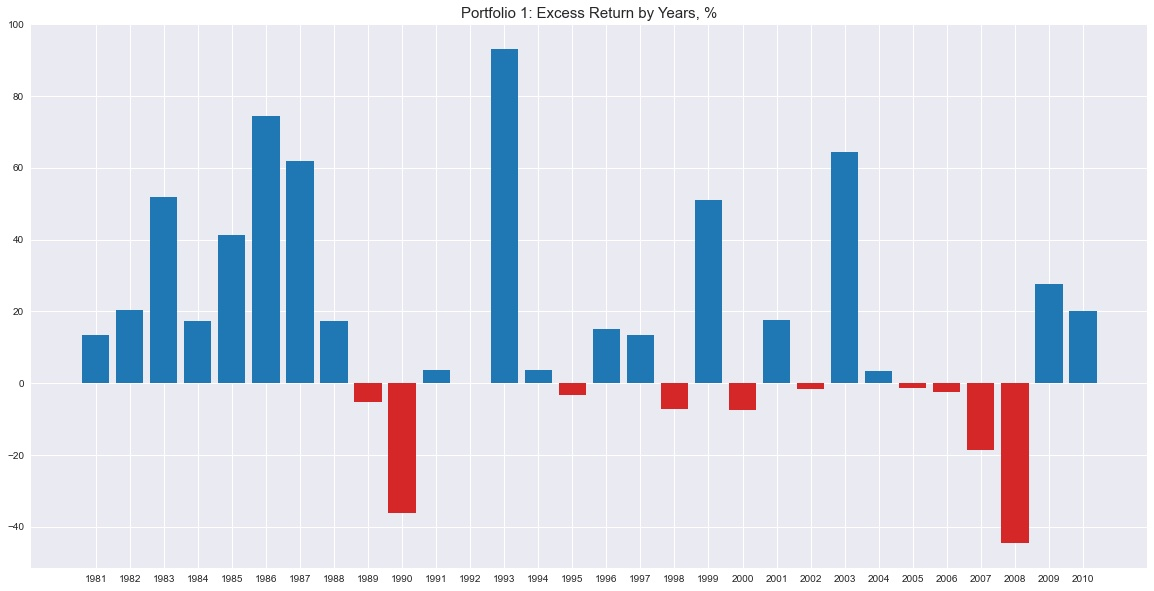
\includegraphics[width=\textwidth]{ex_ret_by_years1.jpg}
        \caption{Excess Return by year for portfolio 1}
        \label{fig:ex_ret_by_years1}
    \end{subfigure}
    \hfill
    \begin{subfigure}[b]{0.5\textwidth}
        \centering
        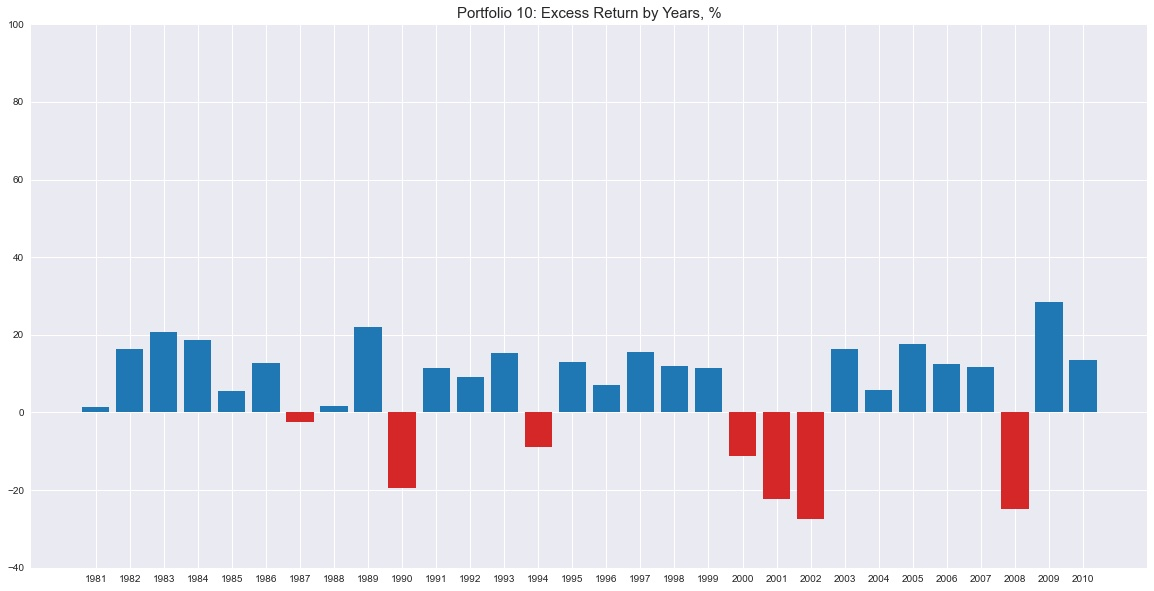
\includegraphics[width=\textwidth]{ex_ret_by_years10.jpg}
        \caption{Excess Return by year for portfolio 10}
        \label{fig:ex_ret_by_years10}
    \end{subfigure}
    \caption{Comparison of excess returns by year for Portfolio 1 and 10}
\end{figure}


%------Regressions------%

\section{Regression Analysis}
To Investigate the sensitivity of each portfolio’s excess return to all risk factors we built a regression model for every one. Each model includes a constant 
term and four factors:
\begin{enumerate}
    \item The excess return on the market portfolio, or market risk premium (RMRF);
    \item Small minus big (SMB) is the difference between the returns on a portfolio of small stocks and a portfolio of big stocks;
    \item High minus low (HML) is the difference between the returns on a portfolio of high book-to-market stocks and a portfolio of low book-to-market stocks;
    \item Winners minus losers (UMD) is the difference between the returns on a portfolio of previous 12-month return winners and previous 12-month loser stocks.
\end{enumerate}

The Four-Factor model can be represented as a linear equation as shown below:
\begin{equation}
    R_i = R_f + \beta_1RMRF + \beta_2HML + \beta_3SMB + \beta_3UMD + \epsilon_i
    \label{eq: ffc_eq} 
\end{equation}

The summary of the models of each portfolio is shown on the following table \textbf{\ref{tab:summary_reg}}.

\begin{table}[H]
    \centering
    \tiny
    \begin{tabular}{ccccccccccc}
    \toprule\toprule
    & \textbf{XS1} & \textbf{XS2} & \textbf{XS3} & \textbf{XS4} & \textbf{XS5} & \textbf{XS6} & \textbf{XS7} & \textbf{XS8} & \textbf{XS9} & \textbf{XS10}\\ 
    \midrule
    $R^2$ & 13\% & 11\% & 14\% & 6\% & 16\% & 9\% & 6\% & 12\% & 5\% & 1\% \\
    $Adj. R^2$ & 20\% & 10\% & 3\% & -1\% & 3\% & 19\% & 11\% & 13\% & 20\% & 16\% \\
    Intercept $\alpha$ & 0.005379 & 0.005661 & 0.003544 & 0.002398 & 0.001190 & 0.001816 & 0.001018 & 0.000472 & 0.001168 & -0.000018 \\
    \midrule
    \textbf{RMRF} &  &  &  &  &  &  &  &  &  &  \\
    Beta & 0.669732 & 0.746535 & 0.745864 & 0.808085 & 0.864139 & 0.893728 & 0.924632 & 0.995537 & 1.076245 & 0.955129 \\
    Std. Err. & 20\% & 10\% & 3\% & -1\% & 3\% & 19\% & 11\% & 13\% & 20\% & 16\% \\
    t-value & 13\% & 11\% & 14\% & 6\% & 16\% & 9\% & 6\% & 12\% & 5\% & 1\% \\
    p-value & 20\% & 10\% & 3\% & -1\% & 3\% & 19\% & 11\% & 13\% & 20\% & 16\% \\
    \midrule
    \textbf{SMB} &  &  &  &  &  &  &  &  &  &  \\
    Beta & 0.833417 & 0.895935 & 0.928535 & 1.004553 & 0.904032 & 0.882555 & 0.844916 & 0.724549 & 0.451132 & -0.150017 \\
    Std. Err. & 20\% & 10\% & 3\% & -1\% & 3\% & 19\% & 11\% & 13\% & 20\% & 16\% \\
    t-value & 13\% & 11\% & 14\% & 6\% & 16\% & 9\% & 6\% & 12\% & 5\% & 1\% \\
    p-value & 20\% & 10\% & 3\% & -1\% & 3\% & 19\% & 11\% & 13\% & 20\% & 16\% \\
    \midrule
    \textbf{HML} &  &  &  &  &  &  &  &  &  &  \\
    Beta & 0.104161 & 0.055465 & 0.073296 & 0.106107 & 0.040708 & 0.020540 & 0.016041 & 0.034221 & 0.009106 & -0.008059 \\
    Std. Err. & 20\% & 10\% & 3\% & -1\% & 3\% & 19\% & 11\% & 13\% & 20\% & 16\% \\
    t-value & 13\% & 11\% & 14\% & 6\% & 16\% & 9\% & 6\% & 12\% & 5\% & 1\% \\
    p-value & 20\% & 10\% & 3\% & -1\% & 3\% & 19\% & 11\% & 13\% & 20\% & 16\% \\
    \midrule
    \textbf{UMD} &  &  &  &  &  &  &  &  &  &  \\
    Beta & 0.095220 & 0.029742 & 0.002401 & 0.086681 & 0.053836 & 0.014411 & 0.008724 & 0.045609 & -0.057293 & 0.046646 \\
    Std. Err. & 20\% & 10\% & 3\% & -1\% & 3\% & 19\% & 11\% & 13\% & 20\% & 16\% \\
    t-value & 13\% & 11\% & 14\% & 6\% & 16\% & 9\% & 6\% & 12\% & 5\% & 1\% \\
    p-value & 20\% & 10\% & 3\% & -1\% & 3\% & 19\% & 11\% & 13\% & 20\% & 16\% \\
    \midrule
    \textbf{Constant Value} &  &  &  &  &  &  &  &  &  &  \\
    Beta & 13\% & 11\% & 14\% & 6\% & 16\% & 9\% & 6\% & 12\% & 5\% & 1\% \\
    Std. Err. & 20\% & 10\% & 3\% & -1\% & 3\% & 19\% & 11\% & 13\% & 20\% & 16\% \\
    t-value & 13\% & 11\% & 14\% & 6\% & 16\% & 9\% & 6\% & 12\% & 5\% & 1\% \\
    p-value & 20\% & 10\% & 3\% & -1\% & 3\% & 19\% & 11\% & 13\% & 20\% & 16\% \\
    \bottomrule
    \bottomrule
    \end{tabular}
    \caption{Summary statistics of regressions for every portfolio} 
    \label{tab:summary_reg}
\end{table}

Let us visualize our betas to get a better understanding of the influence of each factor (figure \textbf{\ref{fig:conf_int}}). First we can say that the most significant factors are SMB and RMRF. 
They impact each portfolio’s return. On the other side are the factors UMD and HML. The UMD is significant only for portfolios 4, 9, 10, and the HML - only for portfolio 4.
\begin{figure}[H]
    \begin{center}
        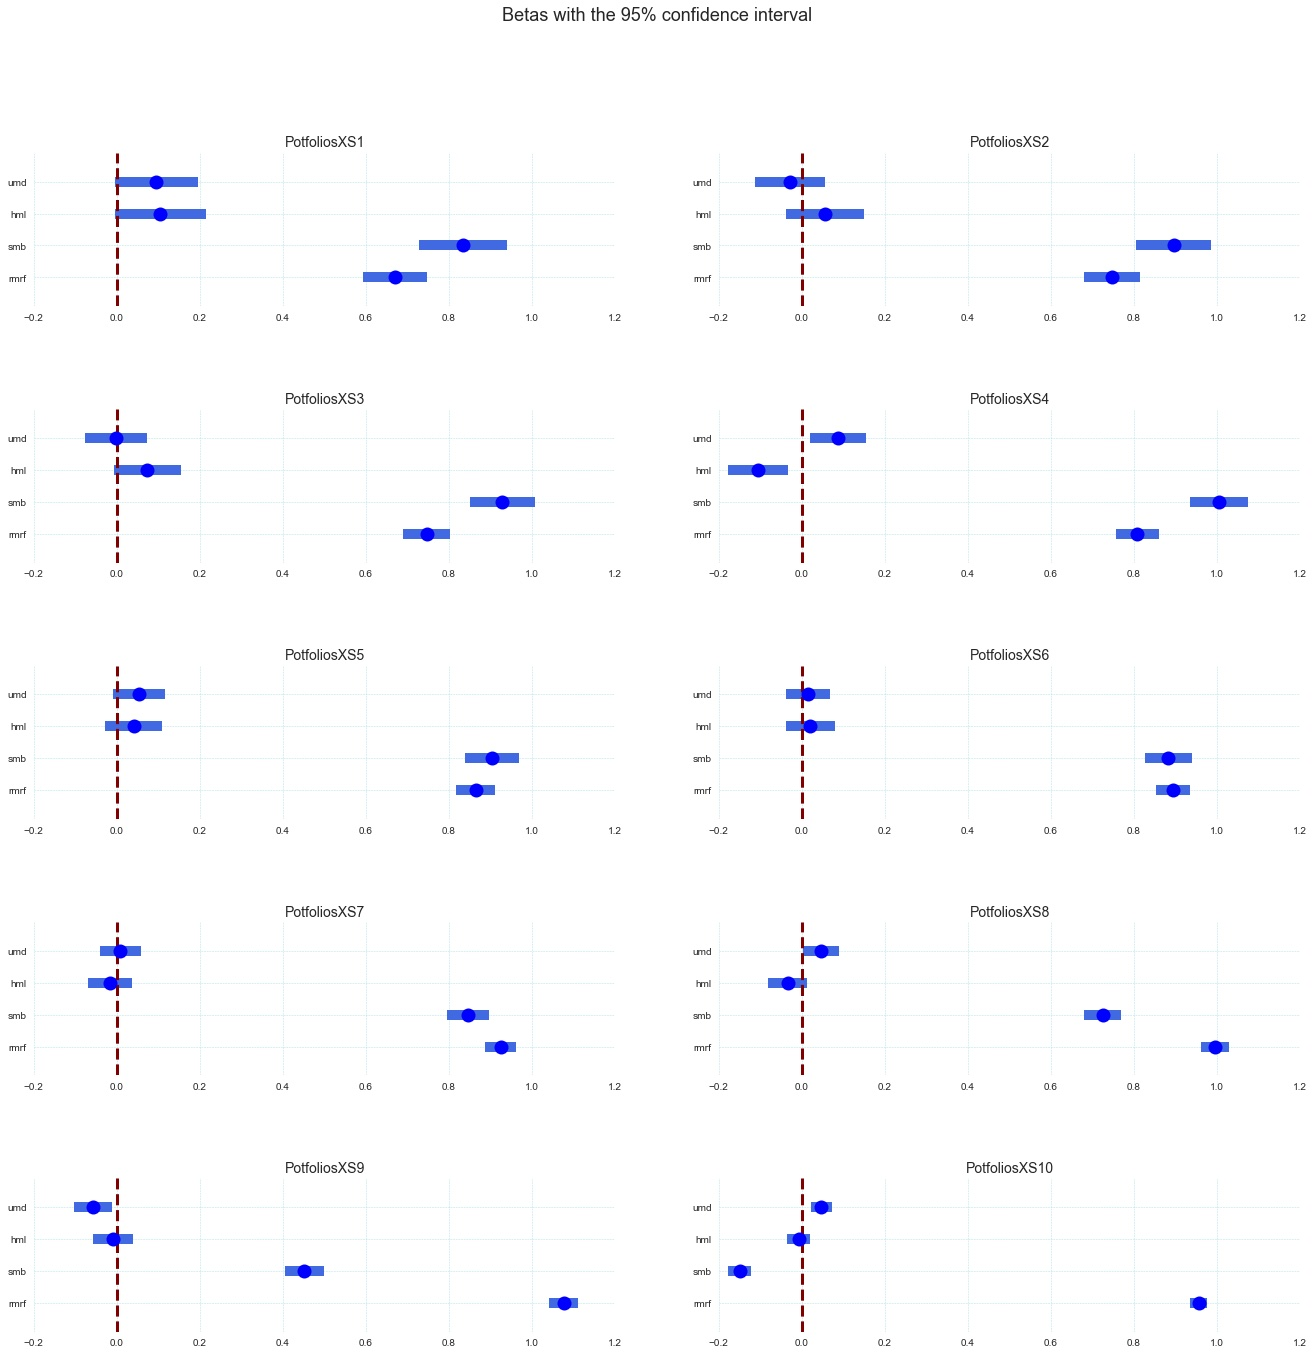
\includegraphics[scale = .3]{conf_int.jpg}
    \end{center}
    \caption{Confidence Interval for every portfolio}
    \label{fig:conf_int}
\end{figure}
When we see the confidence interval of the coefficient is crossing the red line (including the 0) it means that the factor doesn’t impact (or slightly impact) on the asset return.
The highest $R^2$ score has the model of the portfolio 10 - 0,963 (96,3\%). 
An $R^2$ of 100\% means that all movements of a security are completely explained by movements of the factors of our model. It also corresponds with the very 
small standard error, that you can see on the table \textbf{\ref{tab:summary_reg}}. Also we found that portfolio S10 is nearly perfectly correlated (the correlation coefficient is 0,9551) 
with the market returns. We can see it on the figure \textbf{\ref{fig:p10}}. Since the portfolio 10 includes companies with the biggest capitalization, we can make an assumption that 
the market portfolio (rmrf) largely consists of the stocks of the portfolio 10. The smallest R-squared has the portfolio 1 - 60,2\%. So we can say there are other 
factors (aside of our 4 factors) that influence the return of the portfolio 1.

\begin{figure}[H]
    \begin{center}
        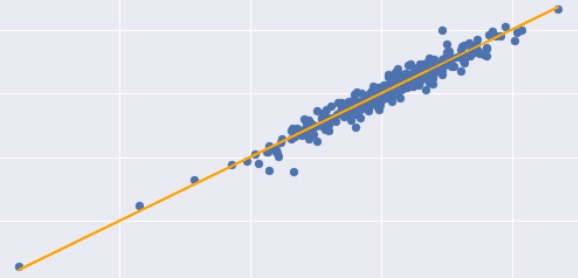
\includegraphics[scale = .7]{p10.jpg}
    \end{center}
    \caption{Correlation of portfolio 10 with RMRF}
    \label{fig:p10}
\end{figure}


\end{document}